\documentclass[10pt,a4paper,twoside,frenchb,english]{book}                % options used for 'Hoofdstuk' or 'Chapter'

%%%%%%%%%%%%%%%%%%%%%%%%%%
%% PACKAGE LOADING TIME %%
%%%%%%%%%%%%%%%%%%%%%%%%%%

%\usepackage{lscape}
\usepackage{pseudocode}
\usepackage{times}      % use Times New Roman Type 1 fonts  (redefines sfdefault,rmdefault,ttdefault)
\usepackage[utf8]{inputenc}
\usepackage[francais]{babel}
\usepackage[T1]{fontenc}

%\usepackage{pslatex}
\usepackage[times]{quotchap}   % fancy chapter beginning
\usepackage{fancyhdr}
%\usepackage[sectionbib]{chapterbib2} % bibliography per chapter
% (sectionbib -> bibliography is \section* instead of \chapter*), should come before babel chapterbib2 
%because local version is 1.9 and solves bug that header was 'References' instead of Chaptername
%\usepackage[sectionbib,numbers,sort&compress]{natbib}  %for citations a la 'Vermeulen et al.' instead of [1]
%\usepackage{tocbibind} % automatically add bibliography, list of figures, ... to table of contents
\usepackage[a4paper,verbose, asymmetric, centering]{geometry}  % better control over margins
%\usepackage[hang]{caption}     %better control over captions (sideways, font, ...)  hang -> 2nd line of caption is indented (caption2 is deprecated and beta)
\usepackage[justification=centering]{caption}     %better control over captions (sideways, font, ...)  
\usepackage{subfigure}  % with scriptsize or so, one can adapt the size
\usepackage{cite}

\usepackage{enumerate}  % to make it possible to define the numbers (A,a, ...)
\usepackage{verbatim}   % extra support for verbatim environments
\usepackage{float}      % you can define 'H' so that floats are forced to be putted 'here'
\usepackage{multirow}   % multirow{nrows}[bigstruts]{width}[fixup]{text} multirow cells
\ifx\pdftexversion\undefined
\usepackage[dvips]{graphicx}
\else
\usepackage[pdftex]{graphicx}
\fi
%\usepackage{psfrag}
\usepackage{chappg}     % page numbering (chapno-pageno), for ToC
\usepackage{url}        % for better url typesetting
\usepackage{expdlist}   % Expanded description (e.g. better alignement) -> needed for acronym_expdlist package
\usepackage{acronym_expdlist}   % for list of acronyms
\usepackage{hhline}     % generates nicer table lines (without missing pixels) + more flexible
%\usepackage{colortbl}  % for coloured columns
%\usepackage{threeparttable}     % adds the possibility to add footnotes in tables
\usepackage{afterpage}  % adds \afterpage command, which makes it possible to issue \afterpage{\clearpage} which flushes all floats after this page
%\usepackage{amsmath}    % adds extra commands, ao. \text within math environment
\usepackage{amsmath,amsfonts,amsthm}
\usepackage{marvosym}   % for Euro symbol
\usepackage{ifthen}     % ifthenelse command
%\usepackage{mathenv}	% better eqnarray
\usepackage{listings}


%%%%%%%%%%%%%%%%%
%% PAGE LAYOUT %%
%%%%%%%%%%%%%%%%%

%%%%%%%%%%%%%%%%%%%%%%%%%%%%%%%%%%%%%%%%%%%%%%%%%%%%%%%%%%%%%%%%%%%%%%
% document: page_layout_definition.tex
%
% last modified: $Id: page_layout_definition.tex,v 1.1 2005/11/18 11:49:23 bvolckae Exp $
%UPDATED ON 05/02/2014 BY SEVENOIS RUBEN TO KEEP COMPATIBILITY WITH NEWER PACKAGE VERSIONS
%
% author: Filip De Turck, Stefaan Vanhastel, Bart Duysburgh, Brecht Vermeulen, Bruno Volckaert, Steven Van den Berghe
%%%%%%%%%%%%%%%%%%%%%%%%%%%%%%%%%%%%%%%%%%%%%%%%%%%%%%%%%%%%%%%%%%%%%%

%%%%%%%%%%%%%%%%%%%%%%%%%%%%%%%%%%%%%%%%%%%%%%%%%%%%%%%%%%%%%%%%%%%%%%

%
% basic dimensions when printing the small page %
% and by using the geometry package             %

% settings Filip en Stefaan
%\geometry{bottom=4.0cm,rmargin=4.25cm,body={12.5cm,19.5cm}} % 10pt op a4
%\geometry{marginpar=0.0cm,marginparsep=0.0cm,twosideshift=0.0cm}

% new settings (according book pim which was approved by the promotors) by Bart Duysburgh
%\geometry{bottom=5.34cm,rmargin=4.5cm,body={11.5cm,18.92cm}} % 10pt op a4
%\geometry{marginpar=0.0cm,marginparsep=0.0cm,twosideshift=0.0cm}

%\geometry{body={15.5cm,18.92cm}} % 10pt op a4
\geometry{bottom=5.34cm,rmargin=4.5cm,body={11.5cm,18.92cm}} % 10pt op a4
%\geometry{twoside,marginpar=0.0cm,marginparsep=0.0cm}%,twosideshift=0.0cm}

%\geometry{bottom=2.15cm,rmargin=2.5cm,body={14.14125cm,23.6cm}} % 12pt op a4

%%%%%%%%%%%%%%%%%%%%%%%%%%%%%%%%%%%%%%%

\setlength{\textwidth}{13.5cm}
%\setlength{\textheight}{19.5cm}
%\setlength{\topmargin}{0.0cm}
%\setlength{\oddsidemargin}{0.7cm}
%\setlength{\evensidemargin}{0.7cm}
%\setlength{\marginparwidth}{0pt}
%\setlength{\marginparsep}{0pt}

%%%%%%%%%%%%%%%%%%%%%%%%%%%%%%%%%%%%%%%

\renewcommand{\topfraction}{0.8}

%%%%%%%%%%%%%%%%%%%%%%%%%%%%%%%%%%%%%%%

%%%%%%%%%%%%%%%%%%%%%%%%%%%%%%%%%%%%%%
%% change for subfigure
\renewcommand{\subfigcapskip}{0pt}
%%%%%%%%%%%%%%%%%%%%%%%%%%%%%%%%%%%%%%

%%%%%%%%%%%%%%%%%%%%%%%%%%%%%%%%%%%%%%%
% headings %

\fancypagestyle{plain}{
\fancyhf{}
\renewcommand{\headrulewidth}{0pt}
\renewcommand{\footrulewidth}{0pt}}

\pagestyle{fancy}
\fancyhf{} %clear all header and footer fields
\addtolength{\headwidth}{\marginparsep}
\addtolength{\headwidth}{\marginparwidth}

%\renewcommand{\chaptermark}[1]{\markboth{\chaptername\ \thechapter. \ #1}{}}

\renewcommand{\chaptermark}[1]{\markboth{#1}{}}
%\renewcommand{\sectionmark}[1]{\markright{\thesection\ #1}}

%\newcommand\fdtsvrightmarktmp{{\scshape\small Chapter }}
%\newcommand\fdtsvrightmark{{\scshape\small{Acknowledgment}}}
%\newcommand\fdtsvleftmark{{\scshape\small{Dankwoord}}}

\newcommand\oddpageleftmark{}
\newcommand\evenpagerightmark{}

%\fancyhead[LE,RO]{\itshape\bfseries\small\thepage}
%\fancyhead[LO]{\itshape\bfseries\small\leftmark}
%\fancyhead[RE]{\itshape\bfseries\small\rightmark}
\fancyhead[LE,RO]{\small\thepage}
\fancyhead[LO]{\oddpageleftmark}
\fancyhead[RE]{\evenpagerightmark}
%\fancyfoot[C]{\itshape\bfseries\footnotesize \chaptername\ \thechapter}

%%%%%%%%%%%%%%%%%%%%%%%%%%%%%%%%%%%%%%%%%%%%%%%%%%%%


%%%%%%%%%%%%%%%%%%%%%%%%%%%%%%%%%%%%%%%%%%%%%%%%%%%%
% depth of numbering and depth of table of contents %

\setcounter{tocdepth}{3} % titels tot en met niveau subsubsection worden in table of contents opgenomen
\setcounter{secnumdepth}{3} % tot en met niveau subsubsection wordt er genummerd
%%%%%%%%%%%%%%%%%%%%%%%%%%%%%%%%%%%%%%%%%%%%%%%%%%%



%%%%%%%%%%%%%%%%%%%%%%%%%%%%%%%%%%%%%%%%%%%%%%%%%%%
%%%%% Definition for Big letter at the beginning of a paragraph %%
\def\PARstart#1#2{\begingroup\def\par{\endgraf\endgroup\lineskiplimit=0pt}
    \setbox2=\hbox{\uppercase{#2} }\newdimen\tmpht \tmpht \ht2
    \advance\tmpht by \baselineskip\font\hhuge=cmr10 at \tmpht
    \setbox1=\hbox{{\hhuge #1}}
    \count7=\tmpht \count8=\ht1\divide\count8 by 1000 \divide\count7 by\count8
    \tmpht=.001\tmpht\multiply\tmpht by \count7\font\hhuge=cmr10 at \tmpht
    \setbox1=\hbox{{\hhuge #1}} \noindent \hangindent1.05\wd1
    \hangafter=-2 {\hskip-\hangindent \lower1\ht1\hbox{\raise1.0\ht2\copy1}%
    \kern-0\wd1}\copy2\lineskiplimit=-1000pt}
%%%%%%%%%%%%%%%%%%%%%%%%%%%%%%%%%%%%


%%%%%%%%%%%%%%%%%%%%%%%%%%%%%%%%%%%%%%%%%%%%%%%%%%%%
%%% Nog een paar andere zaken  %%%%
%% om een cross-ref naar een voetnoot te kunnen maken definier ik \usefn %%
\newcommand{\usefn}[1]{\mbox{\textsuperscript{\normalfont#1}}}

%\setlength{\captionindent}{1cm}
\renewcommand{\captionfont}{\small \itshape \mdseries \rmfamily}
\renewcommand{\subcapsize}{\footnotesize \itshape \mdseries \rmfamily}

\AtBeginDocument{%
%   \renewcommand{\figurename}{Fig.}%
%   \renewcommand{\tablename}{TABLE}%
   \renewcommand{\tablename}{Table}
  % \renewcommand{\bibname}{References}%
}

%%%%%%%%%%%%%%%%%%%%%%%%%%%%%%%%%%%%%%%%%%%%%%%%%%%



%%%%%%%%%%%%%%%%%
%% HYPHENATION %%
%%%%%%%%%%%%%%%%%

%%%%%%%%%%%%%%%%%%%%
%%  START BOOK    %%
%%%%%%%%%%%%%%%%%%%%

\begin{document}
\graphicspath{{fig/}}
\restylefloat{figure}
\restylefloat{table}

%%   FRONT PAGE       %%
%%%%%%%%%%%%%%%%%%%%%%%%
% 
 \thispagestyle{empty}   % no headings for this page
% 
% % Header
 \noindent
 \begin{minipage}{3cm}%
   \includegraphics*[width=2cm]{UGentlogo}% logo ugent
 \end{minipage}\hfill
 \begin{minipage}{8cm}
 \raggedleft
 \textsf{Ecole Centrale Paris\\
Université Paris-Saclay}
 \end{minipage}
% 
% % Title
\bigskip
   \begin{flushleft}
     \Large \textsf{Production de gaz de synthèse par oxydation partielle à haute pression. \\
Conception et dimensionnement de technologies de combustion.}

   \end{flushleft}
 \hrule
% 
 \bigskip
   \LARGE\noindent \textsf{Arthur Degenève} \hfill
 \bigskip
% 
% % Front Figure
% %\bigskip
% %\begin{figure}[htb]%
% %  \centering%
% %  \includegraphics*[width=\textwidth]{figFront}%
% %\end{figure}%
% %\normalsize
% 
% \bigskip
% \begin{figure}[h!]%
%   \centering%
%   \includegraphics*[height=10cm, keepaspectratio, clip]{figFront}%
% \end{figure}%
 \normalsize
% 
% % Footer
 \vfill
 \begin{minipage}{2.0cm}%
     \includegraphics*[width=2.0cm]{intec}%       % intec logo
 \end{minipage}\hfill
 \begin{minipage}{9cm}
 \raggedleft
 \textsf{Arthur Degenève \\
 Stage master recherche M2: }
 \end{minipage}


%% INFORMATION PAGE     %%
%%%%%%%%%%%%%%%%%%%%%%%%%%

\clearpage{\pagestyle{empty}\cleardoublepage}


\clearpage{\pagestyle{empty}\cleardoublepage}


%% ACKNOWLEDGMENT   %%
%%%%%%%%%%%%%%%%%%%%%%%


\hyphenation{bu-reau-ge-no-ten}
\frontmatter
\chapter{}
\vspace{0.35in}

\selectlanguage{english}

\clearpage{\pagestyle{empty}\cleardoublepage}

%%   TOC, LIST OF FIGURES, LIST OF TABLES, ACRONYMS     %%
%%%%%%%%%%%%%%%%%%%%%%%%%%%%%%%%%%%%%%%%%%%%%%%%%%%%%%%%%%

\renewcommand{\contentsname}{Table of Contents} % original name = Contents

\tableofcontents
\clearpage{\pagestyle{empty}\cleardoublepage}

\listoffigures
\clearpage{\pagestyle{empty}\cleardoublepage}

\listoftables
\clearpage{\pagestyle{empty}\cleardoublepage}

% List of Acronyms
%%%%%%%%%%%%%%%%%%%%%%%%%%%%%%%%%%%%%%%%%%%%%%%%%%%%%%%%%%%%%%%%%%%%%

\chapter*{List of Acronyms}
%     \@mkboth{\MakeUppercase List of Acronyms}%
%              {\MakeUppercase List of Acronyms}%

%\begin{center}
%\textbf{\Large List of Acronyms}
%\end{center}
\textbf{\newline\newline\Large A} \newline
\begin{acronym_expdlist}
\acro{ACE}{Adaptive Communication Environment}
\end{acronym_expdlist}




\clearpage      % clear the current page
\thispagestyle{empty}   % prevent header on this (empty -> next line) page
\mbox{}         % to insert a not empty page, so that there is min. 1 blank page before next chapter
\clearpage{\pagestyle{empty}\cleardoublepage}   % clear the current page and start on the right side

%\renewcommand{\tablename}{Table}

%\renewcommand{\bibname}{References}     % instead of Bibliography
%\renewcommand\citeform{\thechapter.}
%\addcontentsline{toc}{section}{\listfigurename}   % not really sure


%% THE BOOK ITSELF   %%
%%%%%%%%%%%%%%%%%%%%%%%
\mainmatter     % related to chappg numbering
\selectlanguage{english}

\newcommand\fdtsvrightmarktmp{{\scshape\small Chapter }}
\renewcommand\evenpagerightmark{{\scshape\small\chaptername\ \thechapter}}
\renewcommand\oddpageleftmark{{\scshape\small\leftmark}}

%\addtolength{\headwidth}{\marginparsep}
%\addtolength{\headwidth}{\marginparwidth}

%\newcommand{\tm}[1]{$\mbox{#1}^{\mbox{\emph{\scriptsize TM}}}$}

\baselineskip 13.0pt
\graphicspath{{chapt_dutch/}{intro/}{chapt2/}{chapt3/}{chapt4/}{chapt5/}}

% Header
\renewcommand\evenpagerightmark{{\scshape\small Appendix A}}
\renewcommand\oddpageleftmark{{\scshape\small Grid Computing: The Next Network Challenge!}}

%\renewcommand{\bibname}{References}

\hyphenation{}

\chapter[Appendice 1]%
{Appendice 1}
\label{app1}


\emph{
abstract
}

\section{Introduction}
Start text here...



\clearpage{\pagestyle{empty}\cleardoublepage}



% Header
\renewcommand\evenpagerightmark{{\scshape\small Grid Monitoring}}
\renewcommand\oddpageleftmark{{\scshape\small Chapter 2}}

\renewcommand{\bibname}{References}

\hyphenation{}

\chapter[Premières réflexions]%
{Premières réflexions}
\label{premieres_reflexions}

\section{Besoins industriels d'Air Liquide}
Aujourd'hui, les règles de dimensionnement des fours ATR et POX sont mal maîtrisées. Développée par Lurgi, l'ingénierie des fours ATR/POX d'Air liquide n'est pas encore prédictive et la conception manque d'outils pour dimensionner les brûleurs. Air Liquide veut donc davantage maîtriser les process dans le but de :
\begin{itemize}
\item Augmenter la production en sortie de gaz
\item Maîtriser davantage les rejets
\item Obtenir des syngazs de meilleurs qualités (?)
\end{itemize}

Dans ce but, un pilote a été construit en 2004 à Freiberg, reproduisant les conditions des fours industriels. Ce pilote peut fonctionner en plusieurs configurations, notamment ATR. Il dispose de quelques diagnostics, notamment images de la flamme et bilans de masse entrée/sortie. De nombreux tests ont été conduits sur ce brûleur et ces données sont le point de départ du stage.

A travers ce stage, Air Liquide désire :
\begin{itemize}
\item Obtenir des règles de dimensionnement pour les brûleur ATR : lois d'échelles par des nombres adimensionnés adaptés, justifier des choix technologiques
\item Comprendre le comportement des flammes et les mécanismes responsables
\item Donner de la visibilité au numérique, qui manque aujourd'hui cruellement de données expérimentales pour justifier les modèles
\item Dans les paramètres observés par Air Liquide, la forme de la flamme est primordiale, on cherche à bien maîtriser la température au niveau de l'entrée du catalyseur
\end{itemize}

\subsection{Les brûleurs utilisés}
Le pilote HPPOX peut se mettre en mode ATR et son brûleur porte la dénomination ATR-30norm, ce n'est pas le même brûleur que les brûleurs de production des fours ATR industriels. De part la taille déjà, en revanche, on garde des rapports de géométries similaires, et notamment les angles des aubes à 30 et 20.

\subsection{L'ATR au sein de la R\&D aux loges}

Peu de travaux faits sur les ATR, et la majorité concerne l'équipe MathApp. Les volumes d'ATR vendus sont faibles mais sont toujours des investissements conséquents. Air Liquide s'intéresse de nouveaux aux ATR depuis le rachat de Lurgi mais l'appropriation et la remise en questions de la conception des ATR nécessite du temps.

\section{Déroulé et plans du stage}
\begin{enumerate}
\item Travail de bibliographie sur les fours ATR et l'influence du nombre de swirl
\item Identification des paramètres qui pilotent : Re, Swirl1, Swirl2, rapport impulsion
\item Etude et dimensionnement des brûleurs à utiliser et de leur conception
\begin{itemize}
\item Fabrication industrielle (cas le plus simple et le plus rapide)
\item Faisabilité du prototypage rapide (le cas échéant)
\end{itemize}
\item Pour chaque brûleur :
\begin{itemize}
\item Diagnostics expérimentaux
\item Régimes de flammes
\item Comparaison avec le pilot HPPOX
\end{itemize}
\end{enumerate}

\subsection{Les intuitions initiales Air Liquide}

Au 1er ordre, c'est la diffusion turbulente qui pilote.

Puisqu'on ne peut pas reproduire Freiberg au labo, il faut respecter l'ordre des échelles pour se rapprocher des mécanismes, en particulier regarder l'évolution dans le diagramme Poisot Veynante. On respecterait cette ordre en conservant :
\begin{itemize}
\item Nombres de swirls équivalents
\item Même rapports d'impulsions
\item Même géométrie
\item Même vitesse
\end{itemize}
Du coup avec des valeurs différentes pour :
\begin{itemize}
\item la pression
\item la richesse
\item le nombre de Reynolds
\end{itemize}
Pour ce qui est de la pression et de la densité, on estime que les mécanismes responsable est davantage le gradient de densité, gradient que l'on veut conserver par le biais des températures (à vérifier).

Concernant la richesse, elle est primordiale dans en combustion prémélangée mais nettement moins en diffusion, dans le mesure ou la flamme se fait en particulier à la stoechiométrie. 

En revanche, il n'y aura pas de réaction de réformage car le méthane sera en défaut. Les diagnostics à comparer avec Freiberg seront donc uniquement des visualisations de flammes. Les canaux seront également inversés entre combustibles et oxydants

\section{The scientific strategy of the internship}

\subsection{The mechanisms driving the topology of the flame}

It must be defined whether the topology of the flame depends on the kinetic or the description of the mixture (diffusion and turbulence). Here are the pros and cons :
\paragraph{Turbulence is driving the flame}
\begin{itemize}

\item According to Veynante - Darabiha, the diffusion flame are mostly driven by the turbulence, and the kinetic can considered as infinitely fast. The argument is not fully verified of course here, this is the purpose of the internship of Ru to study the influence of the kinetic on the topology of the flame
\item This is also an the presumption of Bernard Labegorre and Air Liquide to consider that the turbulent diffusion is the 1st parameter to have an influence on the flame
\item When taking into account a better mixture with LES computation, the topology of the flame is closer to the one is HPPOX

\end{itemize}
\paragraph{Kinetic is driving the flame}
\begin{itemize}
\item The article (\# ref Milosavljevic, V. D., Taylor, A. M. K. P., and
Whitelaw, J. H., Imperial College, Department of
Mechanical Engineering report FS/87/35, (1987).) enhances that a high Reynolds or Swirl number can reach the maximum kinetic velocity so that the kinetic will limit the combustion
\item When using kinetic schemes instead of infinite kinetic, the flame is shorter
\end{itemize}

\subsection{Cooperation with Ru}

Ru and I have two approaches than can be gathered. Even if it is not the only task, we both have to reproduce the results of Freiberg burner, me experimentally and Ru through simulation. It the goal is achieved, implying that we have similar flame topologies, flame length and so on, there are benefits to work together :
\begin{itemize}
\item To my concern, if Ru and I have the same topology of flame, then assuming certain hypothesis, I can find back the velocity field through the simulations of Ru
\item To Ru's concern, we can try different experimental configuration to assess the reliability of her simulation
\end{itemize}

\subsection{Les paramètres expérimentaux}
\paragraph{Nombre de swirl}
Le dispositif sera toujours à aubes fixes, on modifiera dans le nouveau bruleur pilote les nombres de swirls en modifiant la répartition des débits axiaux/tangentiels.
Si on voit que c'est un paramètre de premier ordre, on pourra alors proposer de modifier les swirls sur les bruleurs ATR30-norm, ce qui n'a jamais été fait avant.
\paragraph{Nombre de Reynolds}
Sera limité par la capacité du brûleur, on pourra le baisser légèrement mais ce ne sera vraisemblablement pas un paramètre de premier ordre
\paragraph{rapport d'impulsions}
Avec des outils d'analyses dimensionnelles type Vaschi Buckingham, on fera peut-être apparaître ce paramètre. Voir son influence dans la littérature.
\paragraph{Rapport de dillution à l'azote}
Dans la mesure où il n'y aura pas de réactions de reformage, la vapeur d'eau n'intervient pas et on utilisera de l'azote comme diluant. Le rapport de dilution pourra être intéressant pour diminuer la part de méthane, ainsi diminuer la puissance du bruleur tout en conservant les memes vitesses qu'a Freiberg. Ainsi, c'est pour l'instant un paramètre libre qu'on pourra fitter pour s'accorder à la flamme de Freiberg.
\paragraph{Qarl number}

\clearpage


\clearpage{\pagestyle{empty}\cleardoublepage}

\renewcommand\evenpagerightmark{{\scshape\small Scan of the literature}}
\chapter[Scan of the literature]%
{Revue de Biblio}
\label{revue_de_biblio}
\section{Scale-up et lois d'échelles}

\subsection{Le scale-up peut marcher en éloignant le débit transverse}
\cite{shigeru_azuhata_scale-up_study_of_gas_composition.pdf_1986}
Cet article indique que le scale-up peut-être fait si on fait attention au mélange transverse de l'oxydant dans le fuel. Il recommande par exemple d'éloigner fortement l'arrivée d'air transverse comme il le fait avec son brûleur B. 

Comme explication, l'allumage dépend de la pénétration de l'oxydant dans le fuel, à même vitesse un petit brûleur serait favorisé car son diamètre est plus petit (?)

Mais on pourrait également prendre gare à conserver dans le brûleur ce mécanisme.

\subsection{Scale-up with detonation}

\cite{fig_experimental_2016} this article, scale-up has been experimentally studied with detonation flames : with tubes from 5cm to 71cm, the maximum burning velocity has been fitted with a power fit, which has permitted to forecast the burning velocity for the bigger pipe (71cm) before the experimental setup was finished. The accuracy of the prediction is very good. The power of the fit is not given.

But no explanations of the scale mechanisms is given in this article.
\section{Influence of the Reynolds number}

Article \cite{milosavljevic_influence_1990}  says that increasing the Reynolds number shortens the flame length. If it is due to Reynolds number, it can be bad for the internship, otherwise if it depends more on the bulk velocity, then since we will use the same velocities as the HPPOX, it should be ok. 

Internal Air Liquide (\# ref Freiberg) report showed that between 30 and 40 bar, the flame was the same (length, topology, width...).  Here, pressure mainly modifies the Reynolds number.


\section{Influence of the Swirl number}

\subsection{Recirculation}

Recirculation is generally not observed for swirl numbers below 0.4, so most swirl-stabilized burners are designed for swirl numbers greater than 0.6.

\subsection{Solid body rotation}

On a normalement un solid body rotation pour $r<R/2$ \cite{toh_axial_2010} , cela peut monter plus haut si le swirl augmente \cite{durox_flame_2013}.

\subsection{Flame topology}

between two kinds of burners, the flame topologies can vary a lot, even with the same swirl number. It is particularly the case depending on axial/radial swirl. For example, the shapes are very different between \cite{paul_jourdaine_nom_effect_2016} and \cite{durox_flame_2013}.

From an analysis point of view, it clearly shows that the swirl number is not the only adimensional quantity to describe a swirling flow. The quarl angle is another one, but even if with a quarl angle of $0^\circ$, we need another one to describe why we find a peak in Paul Jourdaine's profile and not the ones of Durox.

\subsection{As the increasing of Reynolds narrows the lean limit, the increasing Swirl may narrows the lean limit as well}

When the bulk velocity increases (equivalent to the Reynolds number), the kinetics reaches its limits so that it increases the lean limit (the rise in the Re is not followed by a rise in the kinetics (which has reached its maximum) so that the flame blows out.

It may be the same case with Swirl number \cite{milosavljevic_influence_1990}. Since the rise in Swirl implies a rise in the tangential velocity, once the maximum kinetic velocity is reached, the rise in the Swirl number can only narrows the lean limits. But it does not explain the bulges of the articles in Fig 3 (there are some discrete values of Swirl where the lean limit is very high, and the flame very stable).

\subsection{Central recirculation zone (CRZ) is independent of S}
This is not the case with the flame length! 

L'article\cite{milosavljevic_influence_1990}  fait varier grandement le nombre de swirls, le quarl et le type de brûleurs pour en tirer ces conclusions, for a given equivalence ratio:
\begin{itemize}
\item The recirculation length is independant of the Swirl number, of the bulk injection (equivalent to Reynolds) and of a second order with the type of nozzle used
\item Strongly depends on the quarl number (CRZ increases with the quarl)
\end{itemize}


\subsection{PVC frequency is a linear function of Re}
\cite{martinelli_experimental_2007} According to that article, it is admitted today that the precessing frequency of the PVC is a linear function of the Reynolds number, assuming swirl number S =cste.

\subsection{Using the same adiabatic flame temperature in order to compare different dilutions}
Paul Jourdaine \cite{paul_jourdaine_nom_effect_2016} showed that the topologies of flame are the same between C02 and N2 if the adiabatic flame temperature is respected. The dilution is consequently of second order, this is perfect for the purpose of the internship since it is planned to use another diluent than the PPOX. This is a very powerful results, and the results are still verified if the Swirl number or the quarl number vary.

\section{The quarl angle}

"Ouvreau" in french, the quarl is a piece used in the burner in order to protect the flame from the edge of the burner. One can give a certain angle and \cite{paul_jourdaine_nom_effect_2016} studied the influence of quarl number on a premixed flame. From $0^\circ $ to $45^\circ $, the increase of the quarl number decreases the flame length, and flatten the shape of the flame. Above all, the use of the quarl number is another degree of freedom to shape the flame according to the industrial needs.

According to\cite{milosavljevic_influence_1990}, the CRZ increases as the quarl angles increases.	

\section{Influence of S/C ratio}

According to \# ref Freiberg the flame and the width increases as S/C ratio decreases.

\section{The calculation of the Swirl number}

The only way to be reliable on a Swirl number is to measure it with integration with LDV profile. Since it is not affordable, geometrical approach is necessary to give a 1st value, which can be as false as 100\% error according to the literature.

To do so, the only way is to make assumption on the shape of the velocity field. The calculation of the geometrical swirl number is then only a question of assumption on the shape of the velocity field.

\section{The shape of the velocity field}

If the swirl number is not so important, we can use the results of \cite{durox_flame_2013} to make assumptions, they are very well documented and such shapes of velocity field are quite commonly found in the literature. 

\subsubsection{The Axial Velocity}

If the Swirl number is not high, assuming a constant axial velocity is false but remains the best option and can be quite accurate for low swirl numbers. From now, let us assume $u_{z}=cste$.

\subsubsection{The Tangential velocity}

Three main simple velocity field can be assumed :
\begin{enumerate}
\item $u_{\theta}=cste$ this is currently used but unreliable in the center of the flow, where a discontinuity cannot be possible
\item Solid body rotation : $u_{\theta}=\Omega r$ this is quite almost always true in the center of the flow, and sometimes in the overall flow. But, most of the time, it is completely unreliable when $r \sim R$ 
\item Free vortex flow and conservation of the tangential momentum : $u_{\theta} \cdot r=cste$ This is almost always true near the walls, but unreliable in the center of the flow
\end{enumerate}

\paragraph{Navier-Stokes} I chose to use Navier Stokes cylindrical equations of the tangential velocity to confirm these assumptions. Here are the simplifications :
\begin{itemize}
\item Incompressible
\item independent from $\theta$,$z$ and time $t$, only depends on $r$ coordinate (established flow in a cylinder)
\end{itemize}
Hence, Naviers-Stokes simplifies in :

$\frac{1}{r}\frac{\partial }{\partial r}(r \cdot \frac{\partial u_{\theta(r)}}{\partial r})=\frac{u_{\theta(r)}}{r^2}$ 

Without resolving it, one can see that $u_{\theta}=\Omega r$ and $u_{\theta} \cdot r=cste$ are two particular solutions of the equations. Consequently, in most of the cases, a combination of Solid body rotation and Free vortex flow can well picture the behavior of the swirl, non forgetting that the wall viscosity will eventually drive the tangential velocity to 0 (no matter the assumption on the tangential velocity).

Further investigations will me made to explore if one can fully describe a tangential flow with the following shape : $u_{\theta}=\epsilon_{inner}(r) \Omega r + \epsilon_{outer}(r) \frac{G}{r}$ where $\Omega$ and $G$ are two unknown, and $\epsilon$ the Kronecker symbol. In the center of the vortex, the velocity could be a solid body rotation, and from a certain distance, a free vortex flow.

Nevertheless, we can observe the assumptions in the literature to see that a lot of publications calculates Swirl number without paying enough attention on the shape of the velocity field, and then deplores disparities with the result.

If $u_{\theta}=\Omega r$, then $S=1/2 \frac{u_{\theta}}{u_{z}}$ , and if $u_{\theta}=cste$, then $S=2/3 \frac{u_{\theta}}{u_{z}}$ .

\subsubsection{In case of an axial swirler}
There are two possibilities, listed in the table  :

\begin{tabular}{ l | c | r }
  \hline			
 blade & blade angle depending on $r$ & fixed blade angle \\
  burner & ATR 30norm Freiberg  & Industrial burner \\
  tangential profile & $u_{\theta}(r)=r\Omega$ & $u_{\theta}=cste$ \\
geometrical swirl &  assuming that $\vec{velocity}$ remains parallel to the blade, $S=\frac{1}{2}tan(\alpha(R))$& $S=\frac{2}{3}tan(\alpha)$ \\
  \hline  
\end{tabular}

\subsubsection{With a radial swirler}

\cite{durox_flame_2013} This article tackles the difficulties in determining with accuracy the Swirl number. One can find in the literature many formulas, but each case being different, the only way to know the Swirl number is to measure it (with LDV?). The articles criticizes the fact that many publications does not take care of the accuracy of the swirl number, so that they can be overestimated or underestimated. Depending on the formulas one chooses, there can be error of 100\%. The article study different formulas in a radial swirler, the selected ones at the end are :

\begin{itemize}
\item $S=\frac{1}{4} \frac{R}{L} tan(\alpha)$ where $R$ is the radius of the swirler and $L$ the height of the radial injection. In this formula, one uses the hypothesis of a solid body rotation $u_{\theta}(r)=\Omega r$ and can be easily demonstrated.
\item The other ones $S=0.75\frac{\bar{u_{\theta}}}{\bar{u_{z}}}$ comes from a fit and is very accurate but recquires to know $\bar{u_{\theta}}$
\end{itemize}

But is seems that the common formula from many publications (ref T.C. Claypole, N. Syred, Proc. Combust. Inst. 18 (1981) 81–89. and ref Y. Zhang, D. Shimokuri, Y. Mukae, S. Ishizuka, JSME Int. J. Ser. B 48 (4) (2005)
830–838) : $S=\frac{\pi D D_{0}}{4A_{t}}$. According to my calculation, and to the article (ref T.C. Claypole, N. Syred, Proc. Combust. Inst. 18 (1981) 81–89.), this formula comes from $S=\frac{u_{\theta}(R)u_{z}R^2}{R \cdot u_{z}^2 \cdot R}$ Which is the swirl number without the integral. It is very surprising, and the article \cite{durox_flame_2013} finds that this number is two time larger than the measurements (which would be completely corrected if it would have taken $S=1/2 \frac{u_{\theta}}{u_{z}}=\frac{\pi D D_{0}}{8A_{t}} $, corresponding to a solid body rotation in the center and a free wall vortex near the wall


\subsubsection{With an axial swirler}

The article\cite{palies_combined_2010}  uses an axial swirler and shows the difficulty of calculating a swirl number, a very interesting table compares among different publications the number of swirl, its calculations and the formulas used to compute it. Its own formula to calculate the swirl number is :$S=2/3 tan(\theta)$, and gives 100\% of inacuracy when compared to the integration of LDV profile.

\subsubsection{The strategy for the internship}

Hence, for the purpose of the internship, assuming that LDV is unreachable in Calhory furnace,  here are 3 possibilities to overcome the situation :
\begin{enumerate}
\item With a literary review, try to choose a similar burner to approach the swirl number. Or choose it arbitrarily, knowing that it would be false, but only taking into account it relatively
\item Simulating it on Fluent, with non reacting flow. The difficulty will be to create the geometry of the burner, which is very complicated
\item Use another metric to observe something else on the burner to guess the Swirl number (only possible if scale-up rules are found, or reliable behavior rules of the swirl number)
\end{enumerate}

The main problem is that the rules to compute the swirl number will first depend on the geometry of the burner. One can identify three kinds of swirler : 
\begin{enumerate}
\item the radial swirler : \cite{durox_flame_2013}, the burner with axial and tangential injections
\item the axial swirler : it is the case of the burner ATR-30
\item a mix of the two \cite{paul_jourdaine_nom_effect_2016} as it is the case in OXYTEC, or the pilot we want to build.
\end{enumerate}

To me, the determination of the swirl number must be the most accurate possible. At least, we must fully understand the perimeter of the calculation of the swirl number choosen, these are the very important reasons why I focused on that specific matter :
\begin{enumerate}
\item The whole purpose of the internship is to show that turbulent diffusion is the first parameter who drives the topology of the flame. The industrial parameter we can change is the swirl number through the geometry of the burner. Hence, one cannot neglet the accuracy of the very parameter whose importance is to be proven on the behaviour of the flame.
\item Since we want to prove that pressure and equivalence ratio matter less than swirl and turbulent diffusion, let's be accurate on the swirl geometry!
\item The litterature can give us qui accurate topology of flames according to the swirl number. For instance, one knows that the CRZ is going to appear for S bigger than 0.4-0.6 We cannot content ourself with 100\% inacuray on the swirl number
\item We have two swirl numbers
\item The quality publications check the accuracy of the chosen formula by measuring with PIV/LDV the velocity distribution at the outlet of the burner in order to intergrate them and calculate the quite accurate swirl number. This is not possible in this internship, since we cannot use advanced optical diagnosis.
\end{enumerate}



 





\chapter[Scale-up]%
{Scale-up}
\label{Scale-up}

\section{Analysis of a non reactive flow in a basic case}

\begin{figure}[!h]
  \centering
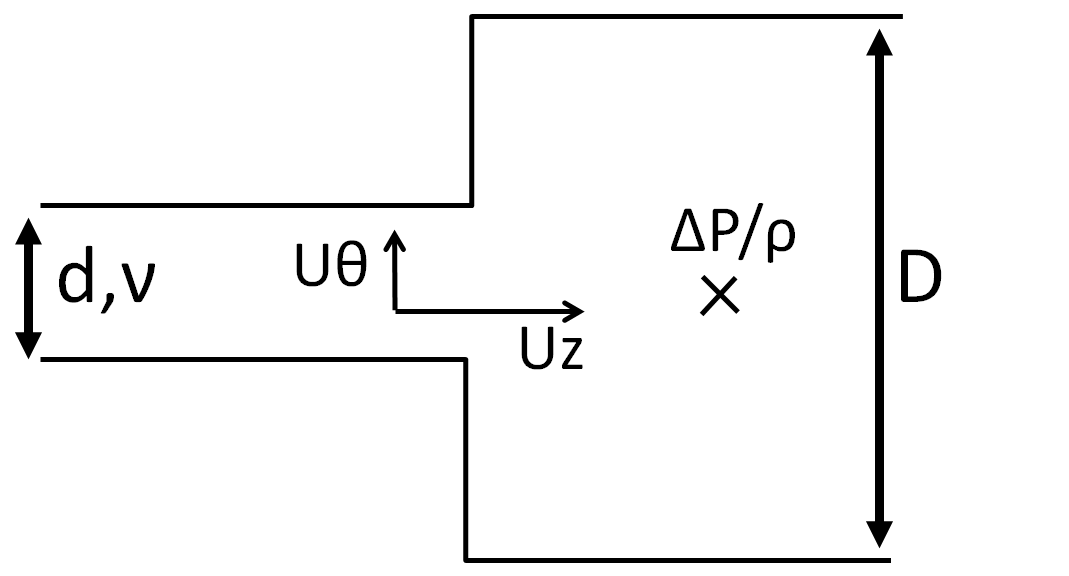
\includegraphics[width=0.6\textwidth]{fig/Schema_Vashy1.png}
  \caption{Basic case}
 \label{Vaschy1}
\end{figure}
Given a burner of internal diameter $d$, with a bulk velocity $u_{z}$,a tangential velocity $u_{\theta}$ ,  followed by a combustion chamber of internal diameter $D$, and a fluid with a cinematic viscosity $\nu$, we what to describe the behavior of the non-reactive flow inside the furnace. For instance, we can study the quantity $\frac{\Delta P}{\rho}$ at a given point inside the combustion chamber, we can otherwise choose $u_{r}$or any physical values, the adimensional numbers will be the same.

We need hypothesis for the velocities : let's assume a top-hat axial velocity, and a solid block body rotation, giving the shape :$u_{\theta}=\Omega r$. Let us use the Vaschy-Buckingham Theorem : we assume that the flow (through the quantity $\frac{\Delta P}{\rho}$ ) only depends on the previous data. 

Since we have 5 independent inputs, with 2 units, there are $5-2=3$ adimensional numbers which fully describes the non-reactive flow. We can guess them, or find it back with linear analysis :
\begin{itemize}
\item $Re$ 
\item $S=\frac{\Omega D}{u_{z}}$
\item $C=\frac{d}{D}$
\end{itemize}
The flow is only a function of $S$, $Re$ and $C$ . The adimensional numbers can vary linearly to these previous quantities, but the combinations of the physical inputs is unique.

\section{In the case of non uniform fields depending on cylindrical coordinates}

\begin{figure}[!h]
  \centering
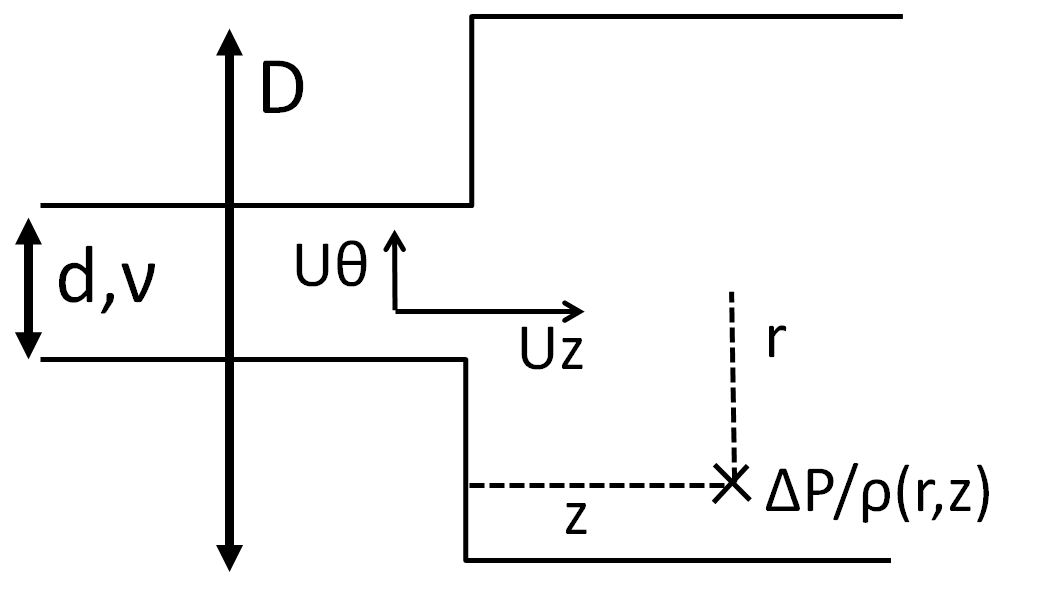
\includegraphics[width=0.6\textwidth]{fig/Schema_Vashy2.png}
  \caption{With cylindrical coordinates}
 \label{Vaschy2}
\end{figure}
In the previous case, the parameter $\frac{\Delta P}{\rho}$ has been considered as a macroscopic one, since not depending on $z$ and $r$ (let us assume the symmetry of rotation by neglecting $\theta$) . Let us now consider the case where we want to study a field depending on cylindrical coordinates : now $\frac{\Delta P}{\rho}(r,z)$. 

If we use the same approach, we easily see that there are 2 more unknown, with the same amounts of units, we have just added two adimensional coordinates to the problem, for instance $r/D$ and $z/D$. The input physical parameters driving the phenomena are the same. Hence, this is not absurd not to consider some coordinates, but we still have to know that the field will depend on adimensional coordinates.

Here, we have : $\frac{\Delta P}{\rho}(r,z)=f(\frac{r}{D},\frac{z}{D},Re,S,\frac{d}{D})$

From now on, let us not consider the dependency of the cylindrical coordinates.

\section{With a quarl angle}

Since Paul Jourdaine \cite{paul_jourdaine_nom_effect_2016} has now shown the huge dependency on the flow of the quarl angle, we can add it in our dimensional analysis.

\begin{figure}[!h]
  \centering
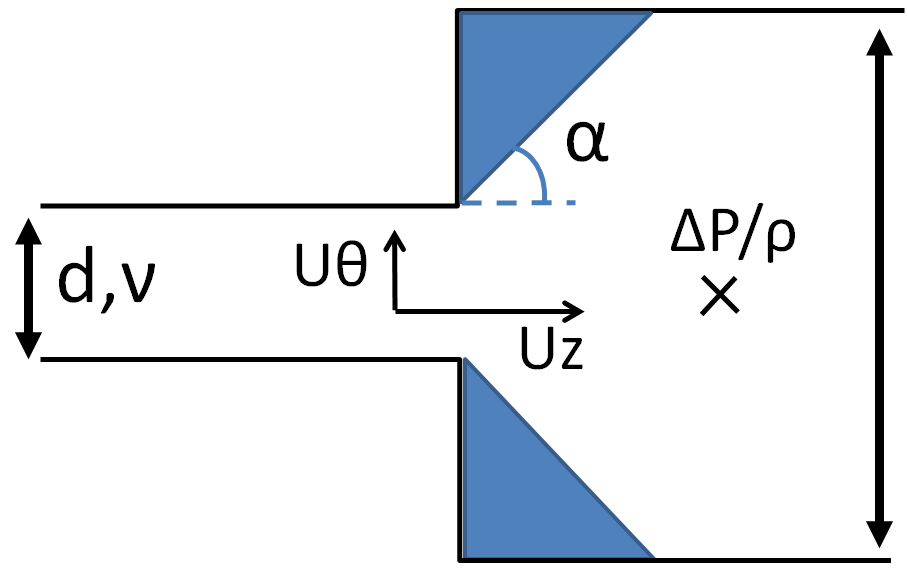
\includegraphics[width=0.6\textwidth]{fig/Schema_Vashy3.png}
  \caption{With quarl angle}
 \label{Vaschy3}
\end{figure}

The Vacshy-Buckingham analysis gives easily : that the quarl number is itself an adimen
sional number, we now have :
$\frac{\Delta P}{\rho}=f(\alpha,Re,S,\frac{d}{D})$



\chapter[Partie filière]%
{Partie filière}
\label{rPartie filière}

\section{Partie filière}

\subsection{Très forte proportion de doctorants}

\subsection{Mobilisation des ressources}
\begin{itemize}


\item Interaction entre deux services MathApp
\item MathApp ou le service combustion peuvent avoir des problèmes pour allouer des ressources (de nombreux projets en cours).
\item Recherche de partenariats au niveau des projets
\end{itemize}



%\addcontentsline{toc}{section}{}


\bibliographystyle{plain}
\bibliography{Zoterobib2.bib}

\end{document}